\documentclass{article} 
\usepackage{geometry}
\geometry{margin=1in}

\usepackage{pgfplots}

\usepackage{amsmath}

\usepackage{xcolor}

\title{STAT 672: Homework \#1}
\author{Tom Wallace}

\setlength{\parindent}{0cm}

\begin{document}

\maketitle

\section*{Problem 1}

\subsection*{A}

See attached code \texttt{hw1\_A.py} for an implementation of rejection sampling
from the unit cube.

\smallskip

The acceptance probability is the volume of an $n$-dimensional ball divided by
the volume of an $n$-dimensional cube:

\begin{equation}
P_{X \sim B^d_\infty}(||X||_2 \leq 1) =
\frac{\mathrm{Vol}(B^d_2)}{\mathrm{Vol}(B^2_\infty)}
= \frac{\frac{\pi ^ {d/2}}{\Gamma(\frac{d}{2} + 1)}}{2^d}
\end{equation}

We know that $\Gamma (n+1) = n!$ Thus, $\Gamma (\frac{d}{2} + 1) = (\frac{d}{2})!$

\smallskip

Stirling's approximation for factorials is useful here.

\begin{equation}
n! \approx \sqrt{2 \pi n}n^ne^{-n}
\end{equation}

Let us consider the case of $2d$. In this case:

\begin{equation}
\mathrm{Vol}(B^{2d}_2) = \frac{\pi ^ d}{\Gamma(d + 1)} = \frac{\pi^d}{d!}
\approx \frac{\pi^d}{\sqrt{2\pi d}d^de^{-d}}
\end{equation}

Rearranging terms, we have:

\begin{equation}
= \frac{1}{\sqrt{2\pi d}} \left( \frac{\pi e}{d} \right)^d
\end{equation}

Referring to $ \left( \frac{\pi e}{d} \right)^d$, the denominator grows (much) faster with $d$ than does the
numerator. As a consequence, if we extend $d$ infinitely, the limit of the ratio is 0.

\begin{equation}
\lim_{d \to \infty} \left( \frac{\pi e}{d} \right)^d = 0
\end{equation}

Which implies:
\begin{equation}
\lim_{d \to \infty} \frac{1}{\sqrt{2\pi d}} \left( \frac{\pi e}{d} \right)^d =
	\frac{1}{\infty} \times 0 = 0
\end{equation}

Returning to (1), we compute the the volume of the unit cube as $d \to \infty$.

\begin{equation}
\lim_{d \to \infty} 2^{2d} = \infty
\end{equation}

So, the ratio of the unit sphere to the unit cube is:

\begin{equation}
\lim_{d \to \infty} \frac{\mathrm{Vol}(B^d_2)}{\mathrm{Vol}(B^2_\infty)} =
\frac{0}{\infty} = 0
\end{equation}

Since this ratio also is the probability of accepting a sample in a rejection sampling
scheme, our expected runtime to generate a single random vector from $\mathrm{B}^d_2$ with
rejection sampling grows asymptotically with $d$. For example, for $d=10000$, our
program would run for a very, very, \textit{very} long time. 

\subsection*{B}
See attached code \texttt{hw1\_1B.py} for an implementation of polar sampling.

\subsection*{C}

The methods implemented in \textbf{A} and \textbf{B} can be empirically
compared. Each program was used to generate 100 samples with $d=10$. The
execution runtime was measured with the Linux \texttt{time} command, e.g.
\texttt{time python3 hw1\_1A.py}. Method B is significantly faster than Method
A, as shown in Table 1.

\begin{center}
	\begin{table}[h]
		\centering
		\caption{Runtime comparison (seconds)}
		\begin{tabular}{|c c c|}
			\hline
			& \textbf{A} & \textbf{B} \\
			\textbf{real} & 2.131 & 0.744\\
			\textbf{user} & 2.150 & 0.744\\
			\textbf{sys}  & 0.172 & 0.192\\
			\hline
		\end{tabular}
	\end{table}
\end{center}



\section*{Problem 2}

\subsection*{A}

Simulation code is attached as \texttt{hw1\_2A.py}. 

\smallskip

As $d$ grows larger, the frequency of the event $\{||X_+ -
Z||^2_2 \geq ||X_{-} - Z||_2^2\}$ increases. This is somewhat counter-intuitive.
Because $Z$ is drawn from the same distribution as $X_+$, we would expect their
difference $X_+ - Z$ to result in something close to a zero-vector, which should
have a smaller Euclidean norm than that of $X_- - Z$
(since these two have different
means), resulting in \textit{low} frequency of the event. This is true in low
dimensions, but as dimensionality grows, the event occurs with \textit{high}
frequency. Why this counter-intuitive result occurs is explained in \textbf{B}.

\begin{figure}[h!]
	\centering
	\caption{Frequency of event}
	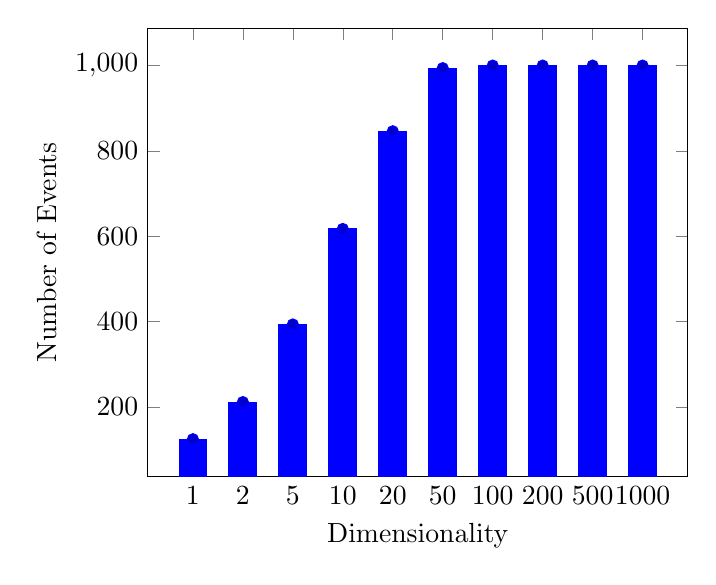
\begin{tikzpicture}
\begin{axis}[ylabel = Number of Events, 
	     xlabel = Dimensionality,
	     xtick = data,
	     symbolic x coords = {1, 2, 5, 10, 20, 50, 100, 200, 500, 1000}]
	\addplot+[ybar, fill = blue] coordinates { 
	(1, 124) 
	(2, 211) 
	(5, 393)
	(10, 617)
	(20, 846)
	(50, 994)
	(100, 1000)
	(200, 1000)
	(500, 1000)
	(1000, 1000)};
\end{axis}
\end{tikzpicture}
\end{figure}

\subsection*{B}

$$ E[||X_+ - Z||^2_2] $$
$$ = E[||X_+||_2^2] -2E[X_+^TZ] + E[||Z||^2_2] $$
$$ E[||X_+||^2_2] = ||\mu_+||^2_2 + tr(\Sigma_+) = 25 + 4d$$
$$ E[||Z||^2_2] = E[||X_+||^2_2] = 25 + 4d$$
$$
E[X_+^TZ] = E[X_+^T]E[Z] = ||\mu_+||^2 = 25
$$
$$
E[||X_+ - Z||^2_2] = 2(25+4d) - 2(25) = \boxed{8d}
$$

\medskip

$$ E[||X_- - Z||^2_2] $$
$$ = E[||X_-||_2^2] -2E[X_-^TZ] + E[||Z||^2_2] $$
$$ E[||X_-||^2_2] = ||\mu_-||^2_2 + tr(\Sigma_-) = 25 + d$$
$$ E[||Z||^2_2] = 25 + 4d$$
$$ E[X_-^TZ] = E[X_-^T]E[Z] = -25$$
$$E[||X_- - Z||^2_2] = (25+d) - 2(-25) + (25+4d) = \boxed{100+5d}$$

\medskip

This theoretical result explains our empirical observations in \textbf{A}. With
low dimensionality, the expected value of $||X_{-} - Z||_2^2$ is greater than
that of $||X_+ -Z||^2_2$, and so our event occurs with low frequency.
However, the expected value of $||X_+ -Z||^2_2$ grows faster with $d$, and so in
high dimensions, our event occurs with high frequency. In essence,
concentration of measure / curse of
dimensionality magnify the effect of $X_+$'s higher variance as dimensionality
grows higher. The different rate of
growth of expected value with $d$ is visualized below in Figure 2.

\begin{figure}[h!]
	\centering
	\caption{Change in expected value with $d$}
	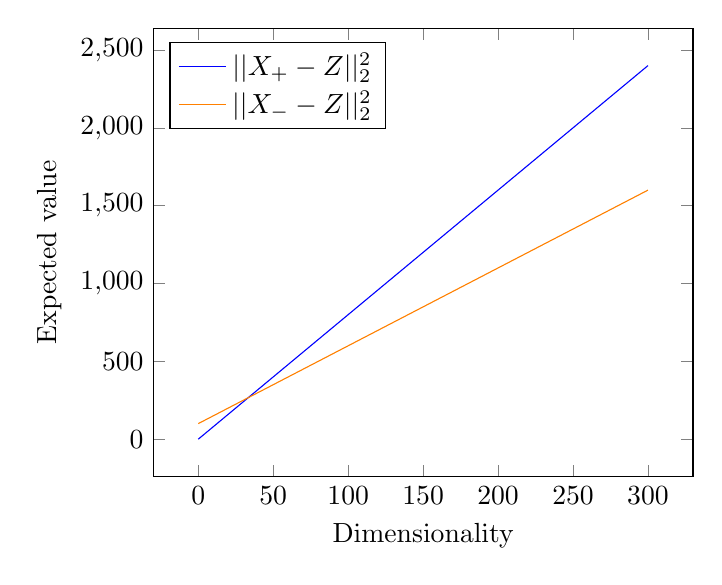
\begin{tikzpicture}
\begin{axis}[ylabel = Expected value, 
	     xlabel = Dimensionality,
	     legend pos = north west]
	     \addplot[domain=0:300, color=blue]{8*x};
	     \addlegendentry{$||X_+ - Z||^2_2$}
	     \addplot[domain=0:300, color=orange]{100+5*x};
	     \addlegendentry{$||X_- - Z||^2_2$}
\end{axis}
\end{tikzpicture}
\end{figure}
\end{document}
